\subsection{Markers Detection}
Markers detection block, can be divided in two parts: \textit{segmentation} and \textit{objects filter}.
%
Algorithm makes the detection through the following process:
%
\begin{enumerate}
  \item Get each frame from video input.
  \item Take a frame and segment it using Otsu's threshold.
  \item Detect markers from segmented image.
  \item Write detected markers position in an XML file.
  %\item Se escribe la posición de los marcadores detectados para este cuadro en un archivo con formato XML.
  \item Take the following frame and repeat process from step two.
\end{enumerate}
%
\subsubsection{Detection stages description}
\textit{Segmentation} block uses thresholds with three class Otsu's method\cite{otsu}.\\
%
\textit{Filtering} stage is just a classification of segmented objects. Since objects to be detected have relatively simple shapes (white circles on dark background) and laboratory conditions are controlled during the capture, this stage does not require to implement a complex algorithm. Particularly, it was implemented a circular object detector based on geometric moments\cite{imageMoments} and an area based filter.
%
\subsubsection{Results}
It was observed that results on segmentation stage strongly depends on capture conditions and calculated threshold. Special care must be taken in capture conditions since if does not meet the established, results are not entirely satisfactory.
On the other hand, if captures are made in the established conditions, obtained results are acceptable (Figure \ref{ejemploabelumbr2}).
\vspace{-0.5cm}
\begin{figure}[ht!]
      \centering
        {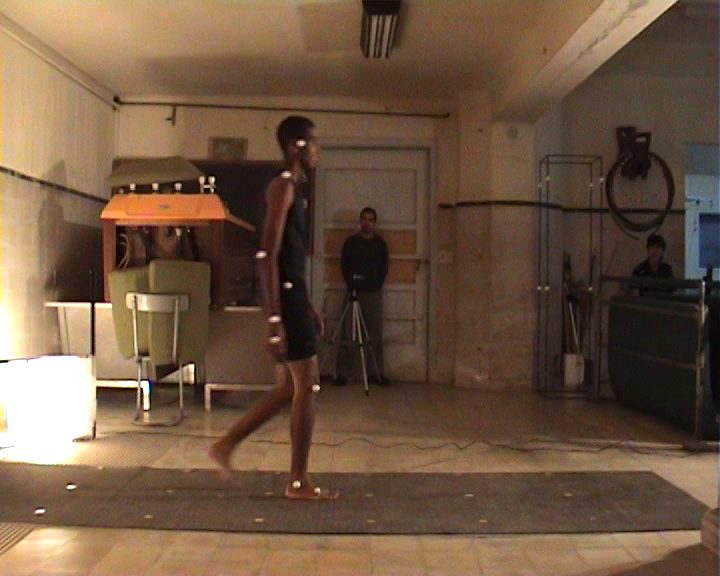
\includegraphics[scale=0.10]{imagenes/abel_original_video.png}\label{abelvideo}}\hspace{1 mm}
        {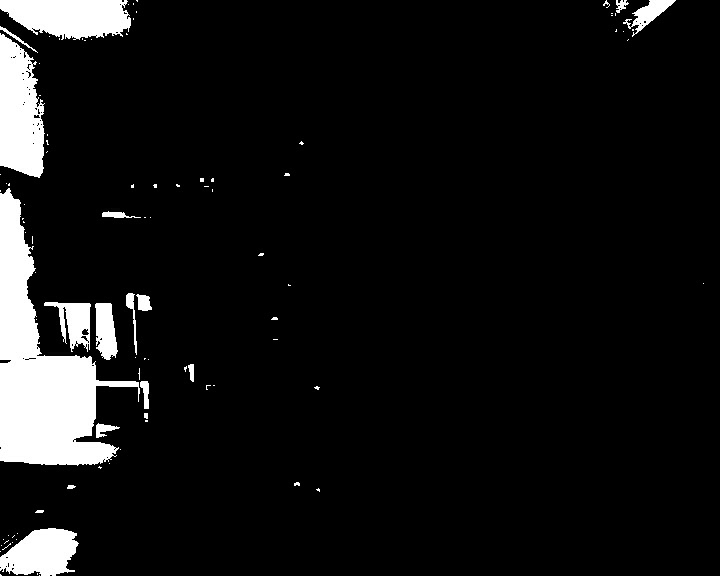
\includegraphics[scale=0.10]{imagenes/abel_original_filtro.png}\label{abelfiltro}}
        {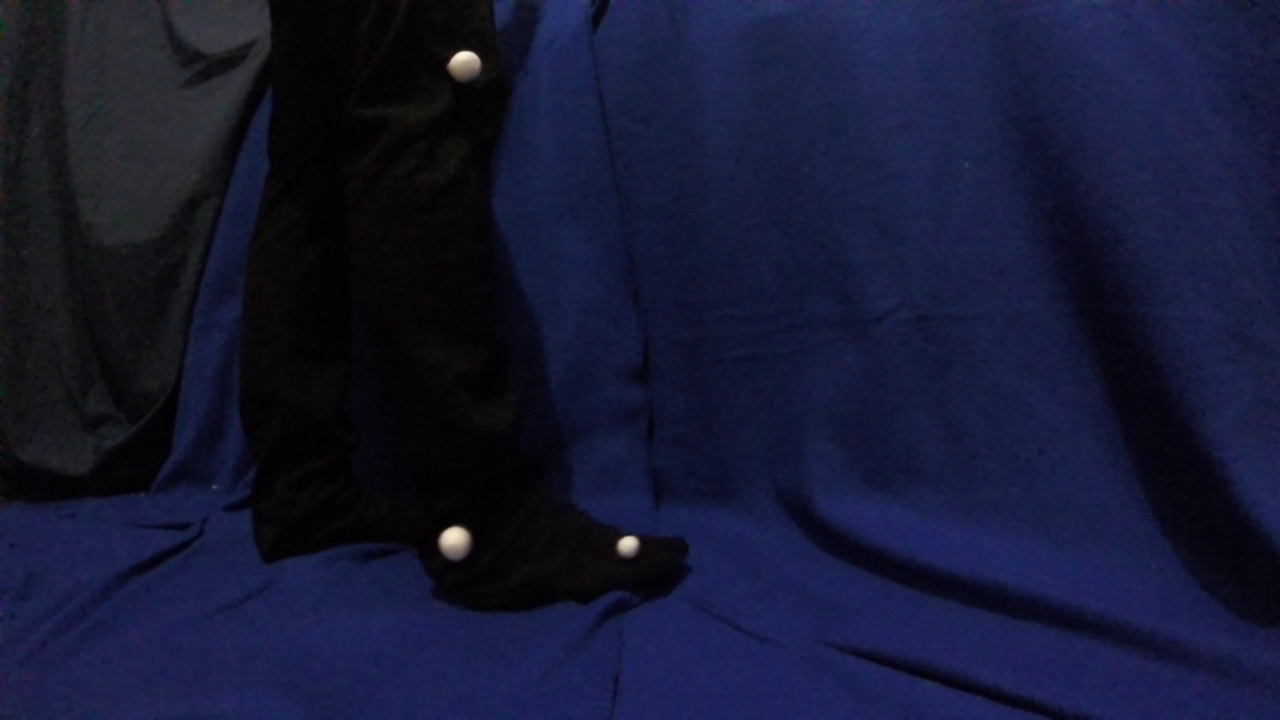
\includegraphics[scale=0.07]{imagenes/orig.png}\label{abelvideo2}}\hspace{1 mm}
       % {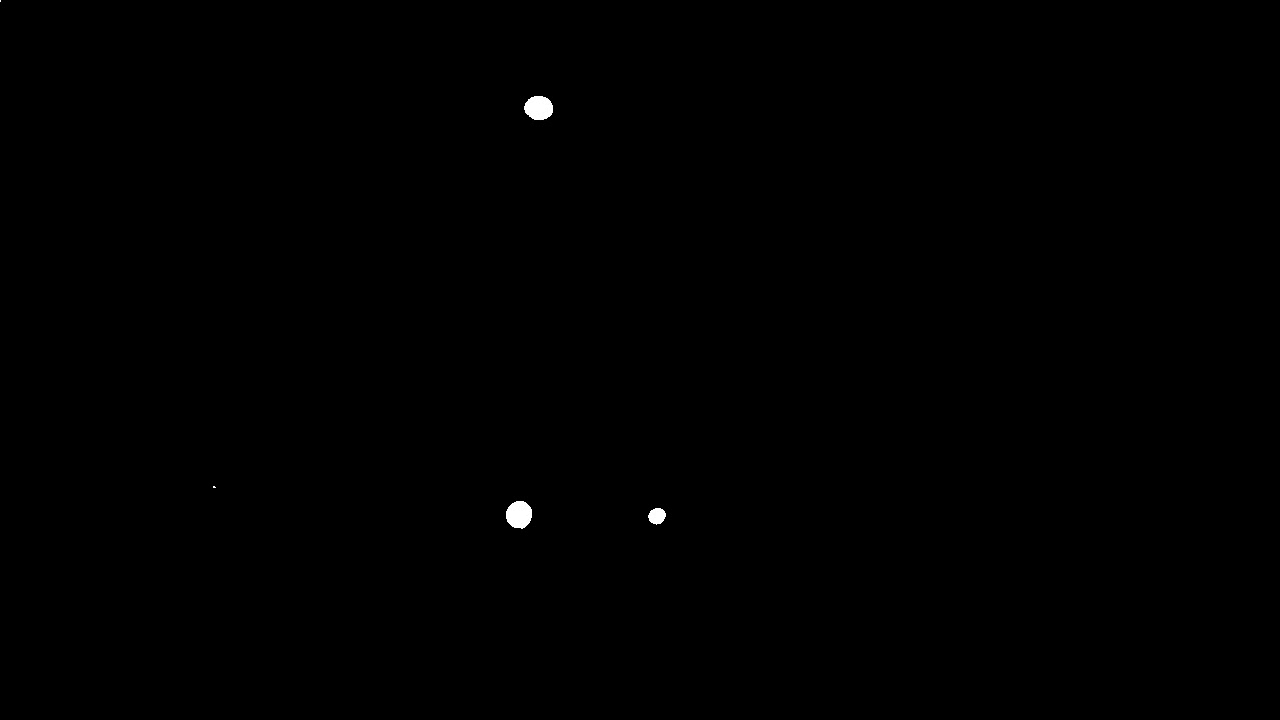
\includegraphics[scale=0.07]{imagenes/filtr.png}\label{abelfiltro2}}\hspace{1 mm}
        {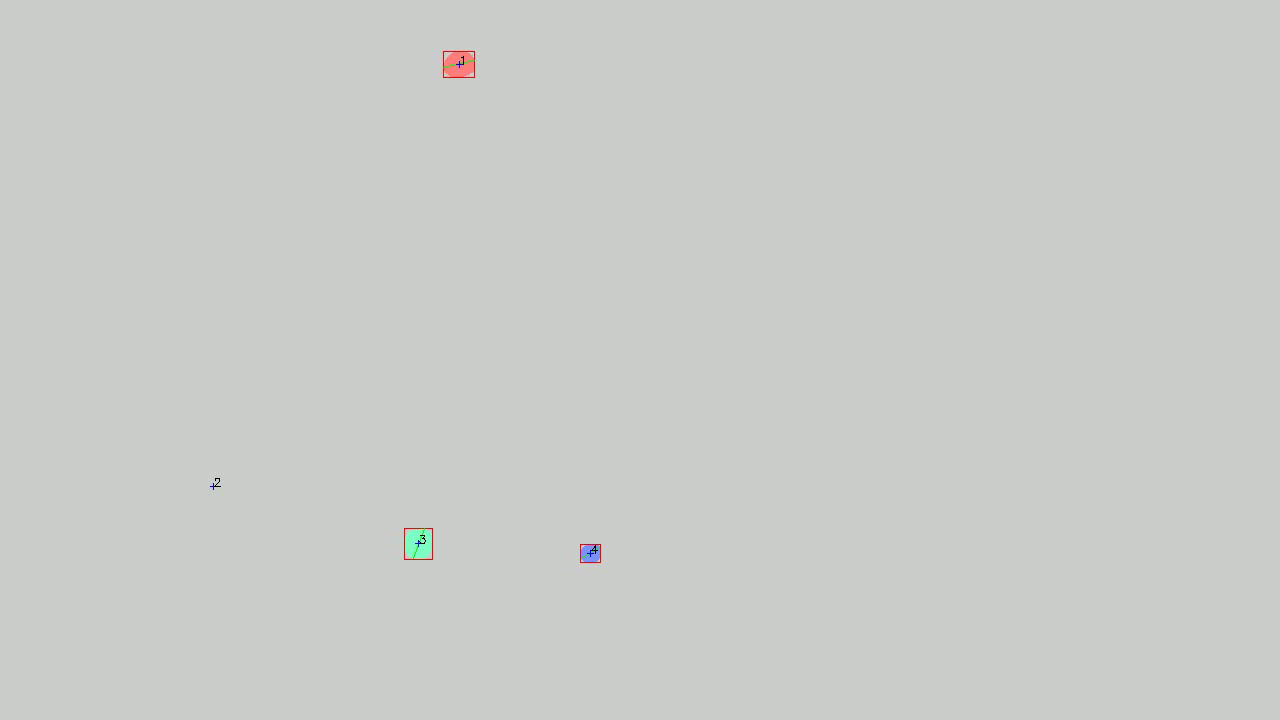
\includegraphics[scale=0.07]{imagenes/detect.png}
        \label{abeldetect}}
      \caption{%Entradas y salidas de cada etapa del bloque de deteción.
       %\textbf{(\ref{abelvideo})} 
       \textit{Left}: original image from a sequencue without capture hypothesis. 
       \textit{Left center}: segmentation results without capture hypothesis.
       % \textbf{(\ref{abelvideo2})} 
       \textit{Right center}: Original capture from a real sequence under capture hypothesis.
       % \textbf{(\ref{abelfiltro2})} Imagen filtrada con el umbral de Otsu. \textbf{(\ref{abeldetect})}
       \textit{Right}: Detected markers.}  
      \label{ejemploabelumbr2}
\end{figure}
%\vspace{-0.6cm}